\chapter*{List of Publications}\label{publications}
\addcontentsline{toc}{chapter}{List of Publications}
\setheader{List of Publications}


%% We use the 'etaremune' environment (the reverse of 'enumerate') to get a
%% numbered list of publications in reverse chronological order. If the list of
%% authors is long, it might be useful to emphasize your own name with \textbf.
{
\onehalfspacing

\section*{Peer Reviewed Journal Articles}
\vspace*{1em}
\begin{enumerate}{\small \compresslist
    \item \textbf{P.\ Bajpai}, {M.\ Poschmann}, {M.H.A.\ Piro}, \textit{Derivations of useful partial molar excess Gibbs energy of mixing expressions of common thermodynamic models}, \href{https://doi.org/10.1007/s11669-021-00886-w}{Journal of Phase Equilibria and Diffusion, 42 (2021) 333-347}.
    \item {M.\ Poschmann}, \textbf{P.\ Bajpai}, {B.W.N.\ Fitzpatrick}, {M.H.A.\ Piro}, \textit{Recent developments for molten salt systems in Thermochimica}, \href{https://doi.org/10.1016/j.calphad.2021.102341}{Calphad, 75 (2021) 102341}.
    \item \textbf{P.\ Bajpai}, {M.H.A.\ Piro}, \textit{Corrigendum to `The thermochemistry library Thermochimica'}, \href{https://doi.org/10.1016/j.commatsci.2021.110659}{Computational Materials Science, 198 (2021) 110659}.
    \item {M.H.A.\ Piro}, {M.\ Poschmann}, \textbf{P.\ Bajpai}, \textit{On the interpretation of chemical potentials computed from equilibrium thermodynamic codes: Applications to molten salts}, \href{https://doi.org/10.1016/j.jnucmat.2019.151756}{Journal of Nuclear Materials, 526 (2019) 151756}.
    \item \textbf{P.\ Bajpai}, {D.\ Schwen}, {M.H.A.\ Piro}, \textit{Performance Considerations of Global Optimisation Algorithms for Computing Chemical Equilibrium in Multicomponent Systems}, {In preparation, to be submitted to Journal of Global Optimization}.
    \item \textbf{P.\ Bajpai}, {M.\ Poschmann}, {D.\ Schwen}, {M.H.A.\ Piro}, \textit{Yellowjacket--GEM: A thermodynamic equilibrium solver for multiphysics simulations in MOOSE}, {In preparation, to be submitted to Calphad}.
}
\end{enumerate}

\section*{Peer Reviewed Conference Proceedings}
\vspace*{1em}
\begin{enumerate}{\small\compresslist
    \item \textbf{P.\ Bajpai}, {M.\ Poschmann}, {D.\ Andr\v{s}}, {C.\ Bhave}, {M.\ Tonks} and {M.\ Piro}, \textit{Development of a new thermochemistry solver for multiphysics simulations of nuclear materials}, \href{https://www.tms.org/TMS2020}{TMS 2020 Supplemental Proceedings, TMS 2020  - 149\textsuperscript{th} Annual Meeting \& Exhibition, San Diego, February 23-27, 2020}.
    \item \textbf{P.\ Bajpai}, {M.\ Poschmann}, {D.\ Andr\v{s}} and {M.\ Piro}, \textit{Progress in developing a new thermochemistry code for corrosion modelling and multiphysics simulation of nuclear fuels}, \href{http://cns-annual-conference.org/2019/index.html}{39\textsuperscript{th} Annual Conference of the Canadian Nuclear Society and 43\textsuperscript{rd} Annual CNS/CNA Student Conference, Ottawa, June 23-26, 2019}.
}
\end{enumerate}

\section*{Conference / Workshop Talks \& Posters}
\vspace*{1em}
\begin{enumerate}{\small\compresslist
    \item \textbf{P.\ Bajpai}, {C.\ Bhave}, {M.\ Poschmann}, {D.\ Schwen}, {M.\ Tonks} and {M.\ Piro}, \textit{Yellowjacket Gibbs Energy Minimiser: Computing Thermochemical Equilibrium for Multiphysics Simulations of Molten Salt Reactors}, \href{https://www.cns-snc.ca/event/2022-fuel-conference/}{15\textsuperscript{th} International Conference on CANDU Fuel, Ajax, Canada, August 21-24, 2022.}.
    \item \textbf{P.\ Bajpai}, {C.\ Bhave}, {M.\ Poschmann}, {D.\ Schwen}, {M.\ Tonks} and {M.\ Piro}, \textit{Yellowjacket: Coupling Gibbs Energy Minimisation with Phase Field Method for Corrosion Modelling in Molten Salt Reactors}, {Workshop for the Molten Salt Thermal Properties Working Group, Virtual, November 15-17, 2021}.
    \item \textbf{P.\ Bajpai}, {C.\ Bhave}, {M.\ Poschmann}, {D.\ Schwen}, {M.\ Tonks} and {M.\ Piro}, \textit{Yellowjacket: Coupling Gibbs Energy Minimisation with Phase Field Method for Corrosion Modelling in Molten Salt Reactors}, \href{https://nubu.nu/events/nufuel-workshop/}{NuFuel 2021, Bangor, United Kingdom, March 15-18, 2021}.
    \item \textbf{P.\ Bajpai}, {C.\ Bhave}, {M.\ Poschmann}, {D.\ Andr\v{s}}, {M.\ Tonks} and {M.\ Piro}, \textit{Yellowjacket: A New MOOSE‐based Corrosion Modelling Application for Molten Salt Reactors}, \href{https://www.tms.org/TMS2021}{TMS 2021  - 150\textsuperscript{th} Annual Meeting \& Exhibition, Virtual, March 15-18, 2021}.
    \item \textbf{P.\ Bajpai}, {M.\ Poschmann}, {D.\ Andr\v{s}}, {C.\ Bhave}, {M.\ Tonks} and {M.\ Piro}, \textit{Development of a new thermochemistry solver for multiphysics simulations of nuclear materials}, \href{https://www.tms.org/TMS2020}{TMS 2020  - 149\textsuperscript{th} Annual Meeting \& Exhibition, San Diego, United States, February 23-27, 2020}.
    \item \textbf{P.\ Bajpai}, {M.\ Poschmann}, {D.\ Andr\v{s}} and {M.\ Piro}, \textit{Progress in developing a new thermochemistry code for corrosion modelling and multiphysics simulation of nuclear fuels}, \href{http://cns-annual-conference.org/2019/index.html}{39\textsuperscript{th} Annual Conference of the Canadian Nuclear Society and 43\textsuperscript{rd} Annual CNS/CNA Student Conference, Ottawa, Canada, June 23-26, 2019}.
}
\end{enumerate}


\setboolean{@twoside}{false}

%\newpage
%\dedication{\textbf{P.\ Bajpai}, {M.\ Poschmann}, {M.H.A.\ Piro} \\ \textit{Derivations of partial molar excess Gibbs energy of mixing expressions for common thermodynamic models}\\  \href{https://doi.org/10.1007/s11669-021-00886-w}{Journal of Phase Equilibria and Diffusion, 42 (2021) 333-347}.}
%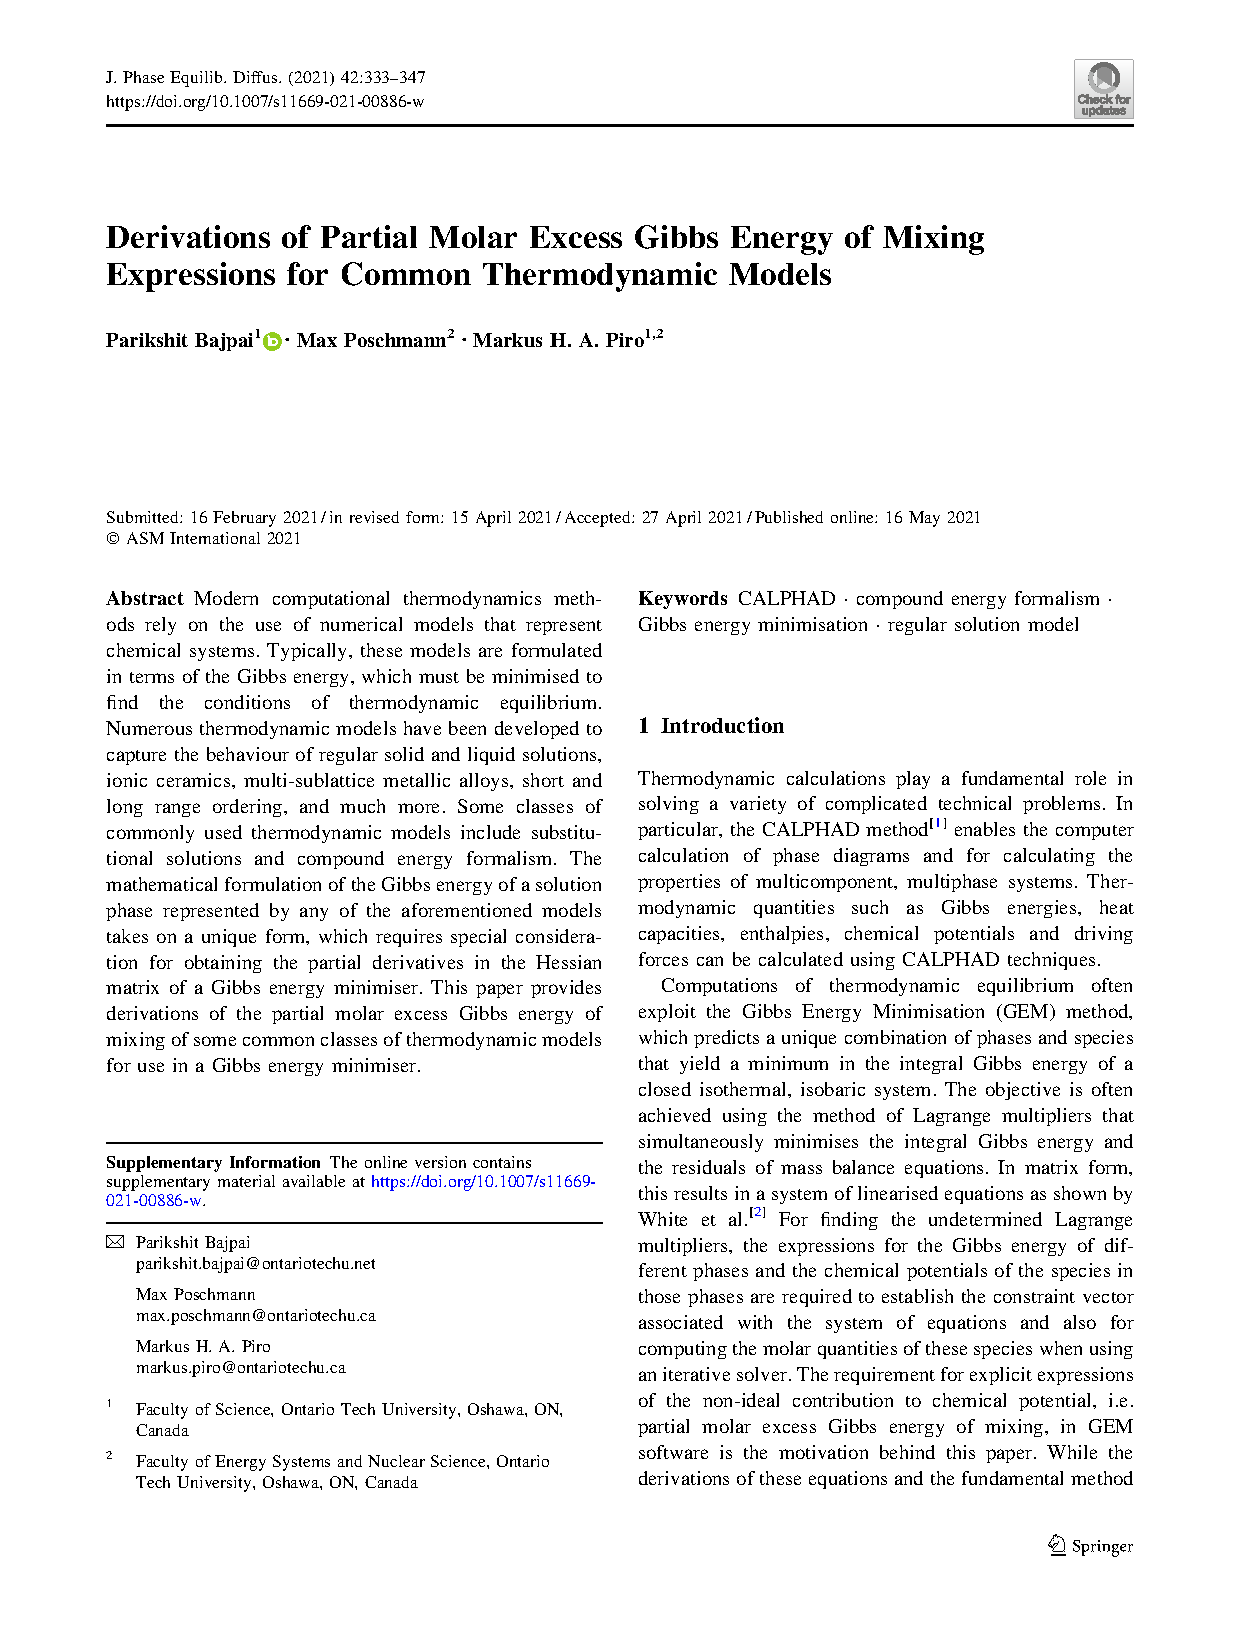
\includepdf[pages=-]{publications/Bajpai_2021_JPED.pdf}
%
%\newpage
%\dedication{{M.\ Poschmann}, \textbf{P.\ Bajpai}, {B.W.N.\ Fitzpatrick} {M.\ Piro}\\ \textit{Recent developments for molten salt systems in Thermochimica}\\ To be submitted to \href{https://www.journals.elsevier.com/calphad}{CALPHAD Computer Coupling of Phase Diagrams and Thermochemistry}. [In preparation]}
%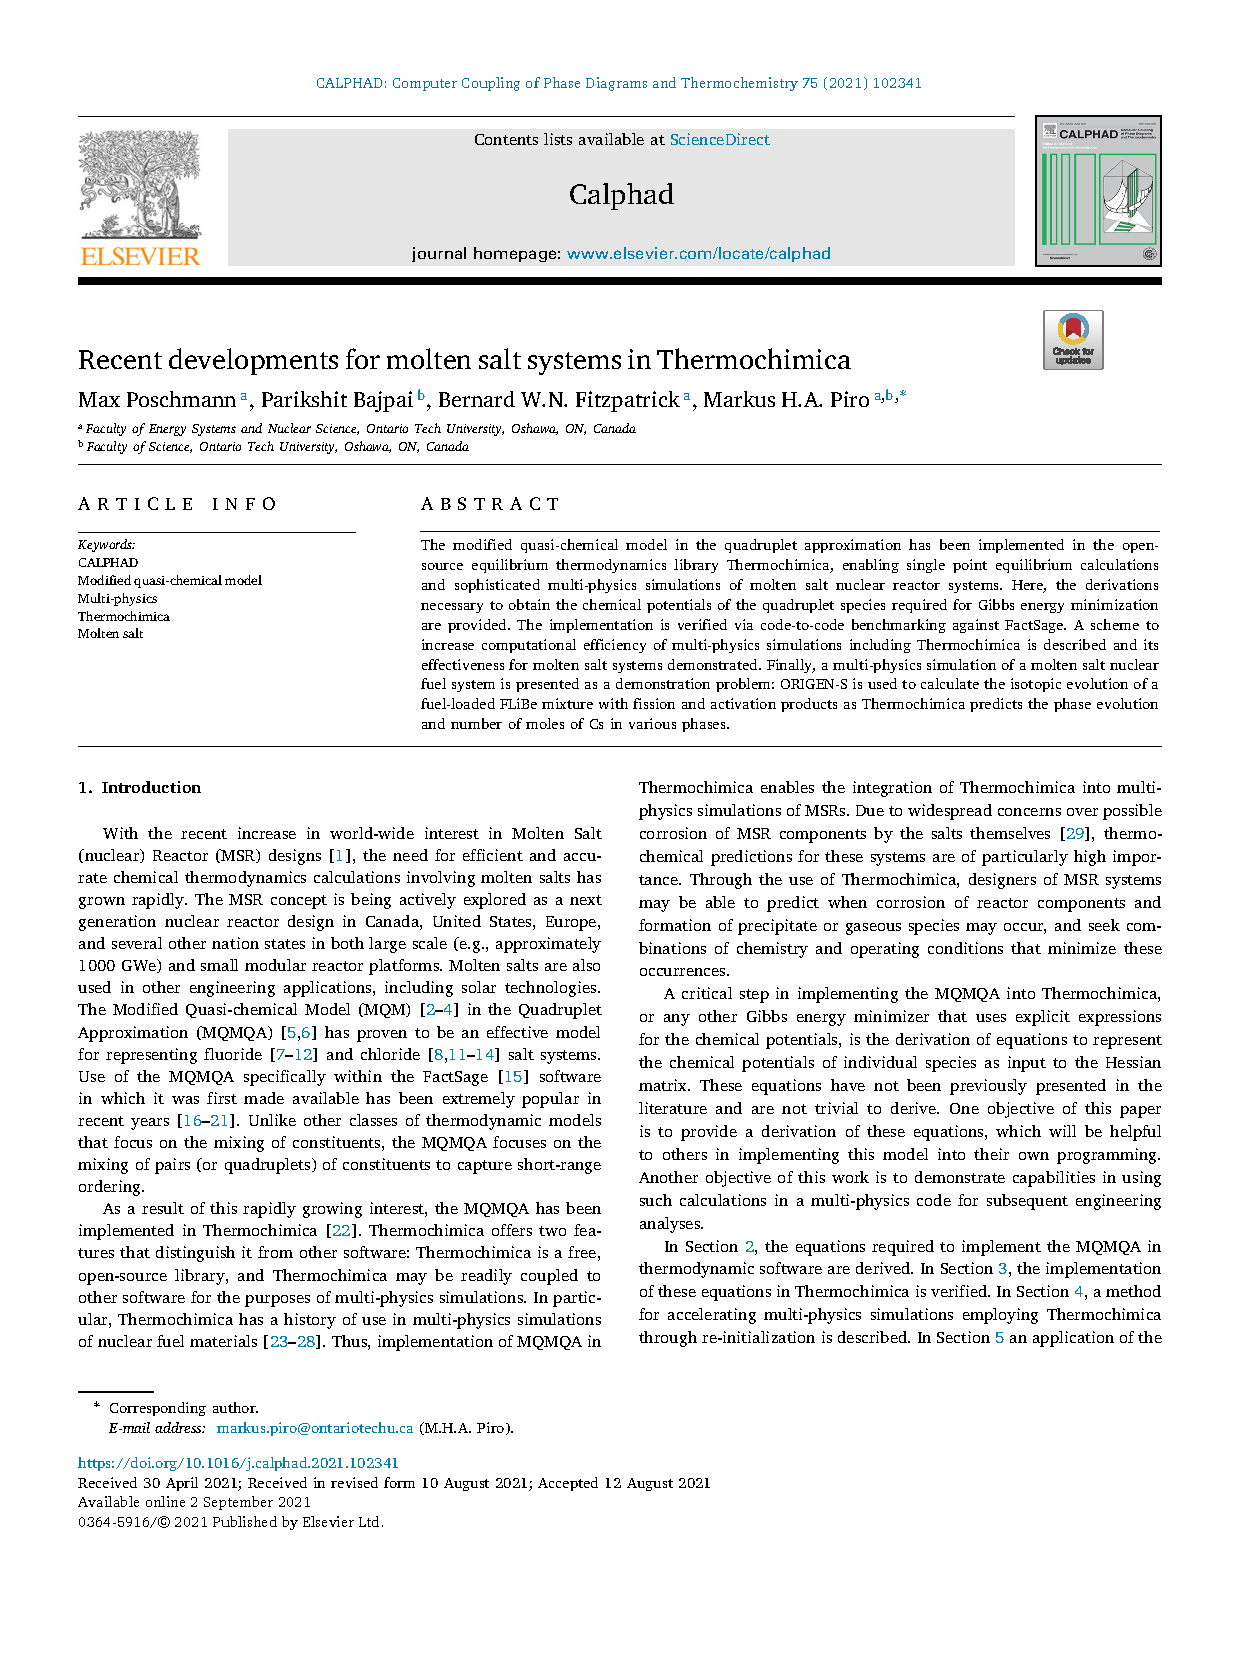
\includepdf[pages=-]{publications/Poschmann_2021.pdf}

%\newpage
%\dedication{{M.\ Piro}, {M.\ Poschmann} and \textbf{P.\ Bajpai} \\ \textit{On the interpretation of chemical potentials computed from equilibrium thermodynamic codes: Applications to molten salts}\\ \href{https://doi.org/10.1016/j.jnucmat.2019.151756}{Journal of Nuclear Materials, 526 (2019) 151756}.}
%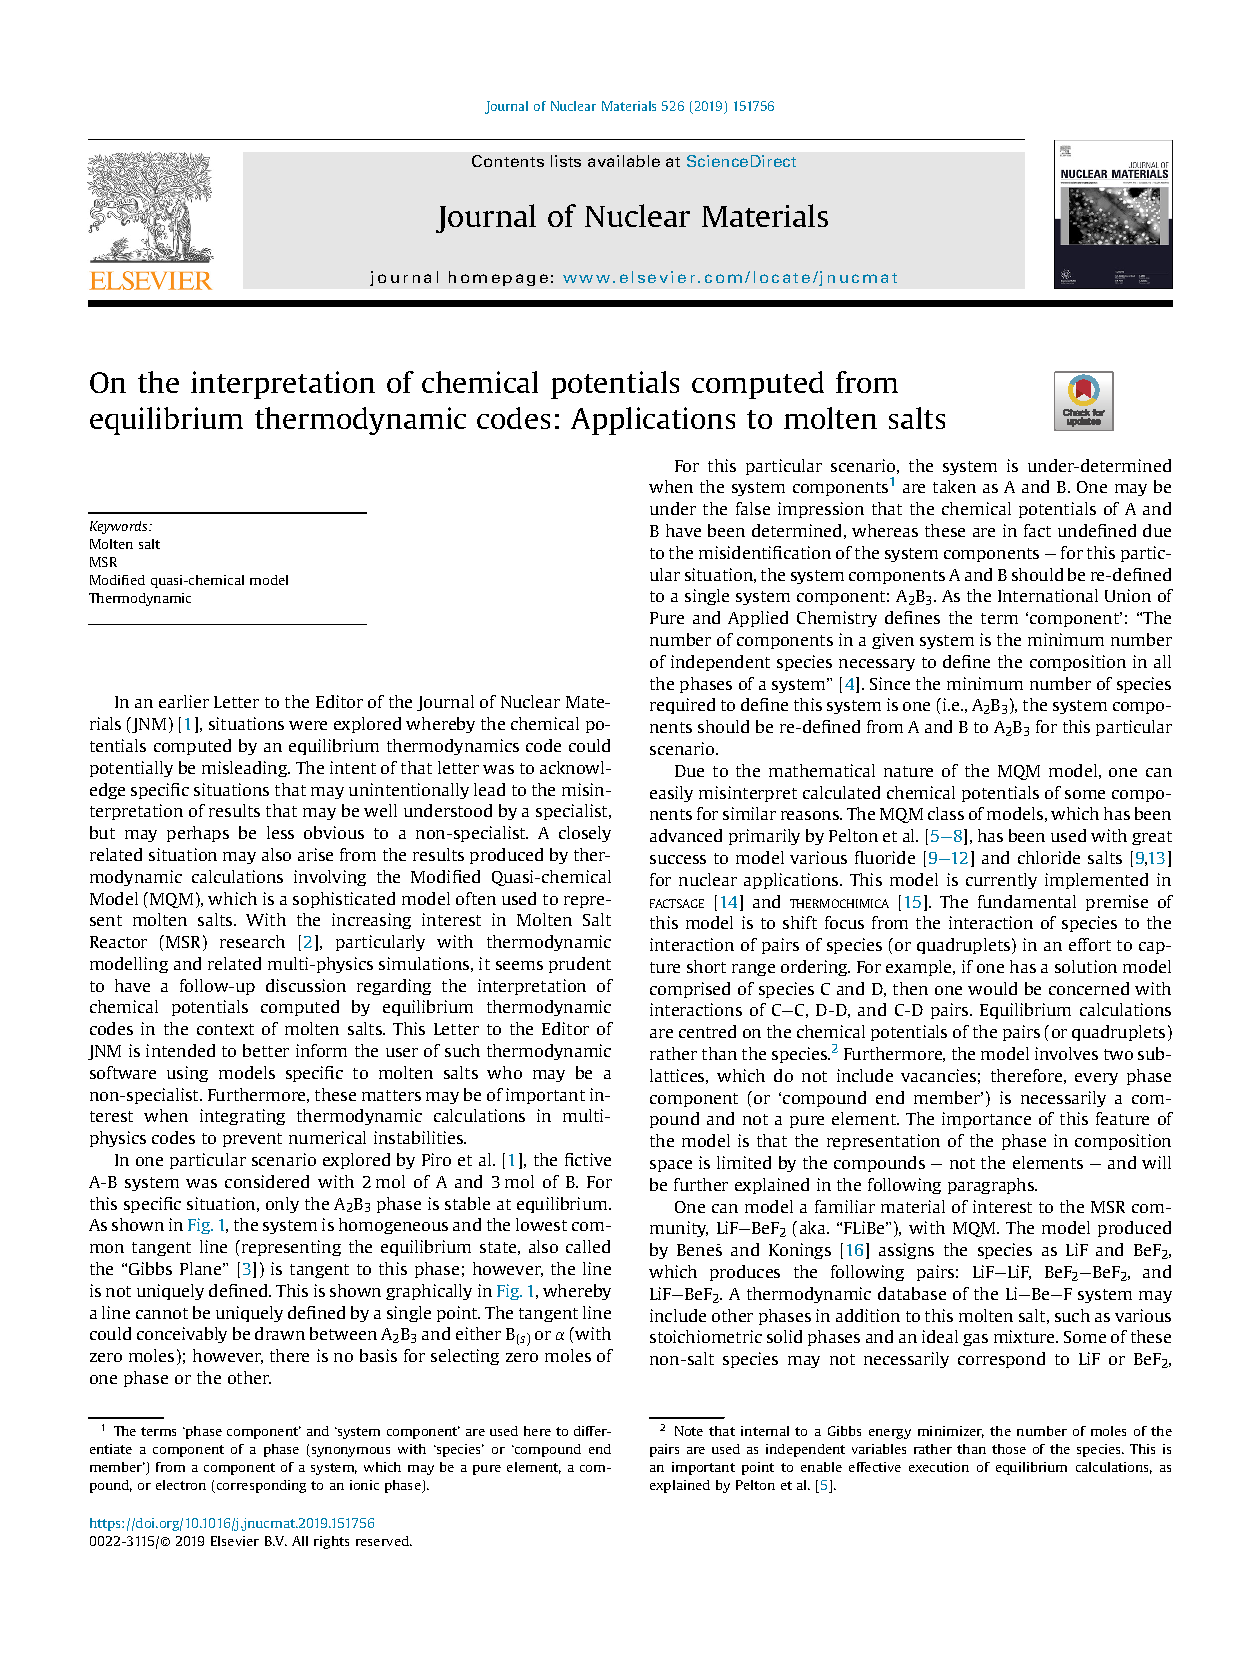
\includepdf[pages=-]{publications/Piro_2019.pdf}
%
%\newpage
%\dedication{\textbf{P.\ Bajpai}, {M.\ Poschmann}, {D.\ Andr\v{s}}, {C.\ Bhave}, {M.\ Tonks} and {M.H.A.\ Piro}\\ \textit{Development of a new thermochemistry solver for multiphysics simulations of nuclear materials}\\ \href{http://https://www.tms.org/TMS2020}{TMS 2020 Supplemental Proceedings, TMS 2020  - 149\textsuperscript{th} Annual Meeting \& Exhibition, San Diego, February 23-27, 2020}.}
%% \includepdf[pages=-]{publications/TMS_2020_Poster.pdf}
%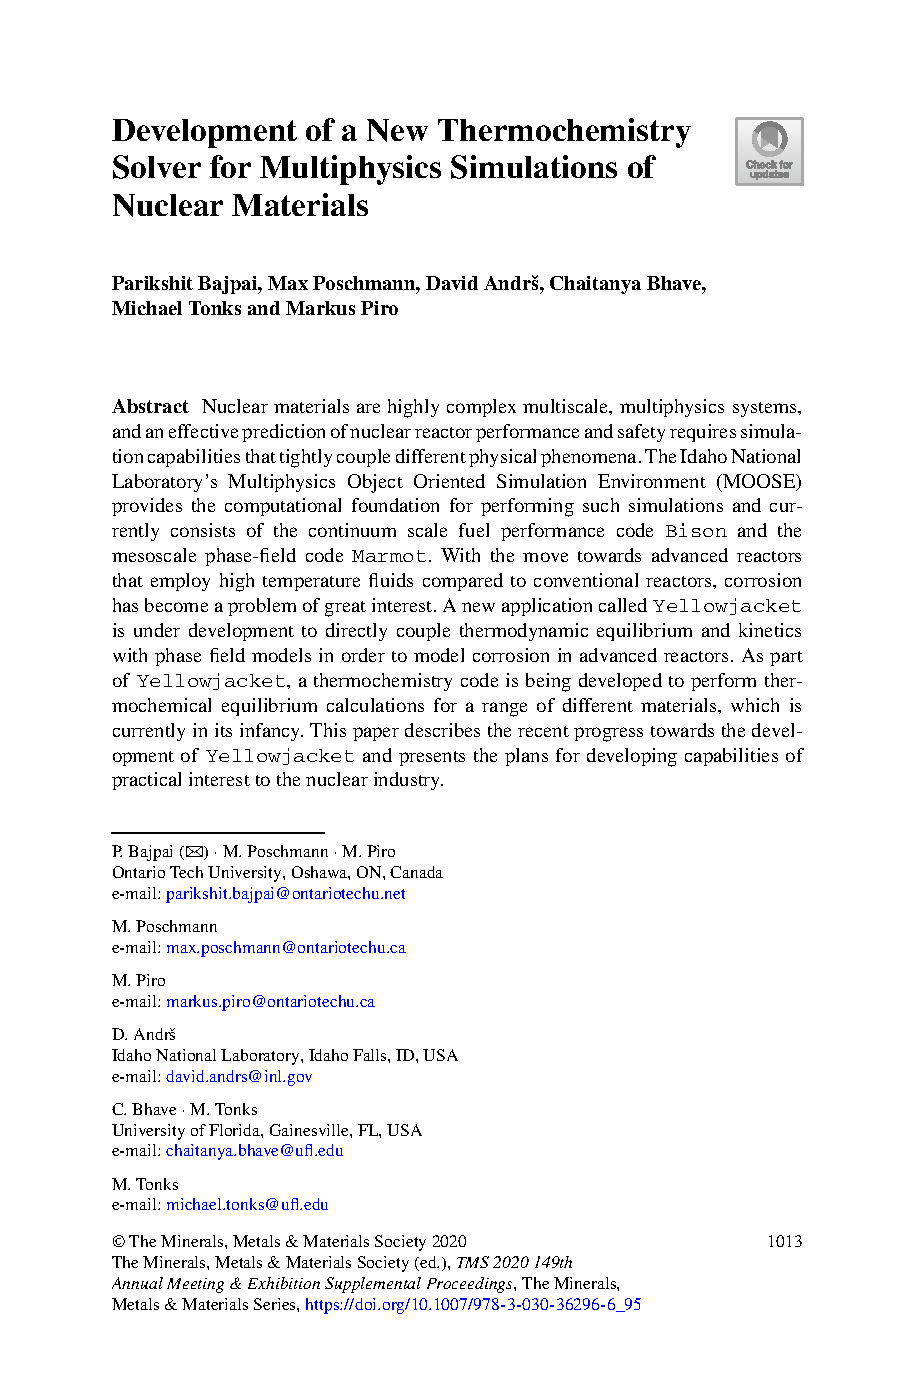
\includepdf[pages=-]{publications/Bajpai_2020_TMS.pdf}
%
%
%\setboolean{@twoside}{false}
%
%\newpage
%\dedication{
%\textbf{P.\ Bajpai}, {M.\ Poschmann}, {D.\ Andr\v{s}} and {M.\ Piro}\\ \textit{Progress in developing a new thermochemistry code for corrosion modelling and multiphysics simulation of nuclear fuels}\\ \href{http://cns-annual-conference.org/2019/index.html}{39\textsuperscript{th} Annual Conference of the Canadian Nuclear Society and 43\textsuperscript{rd} Annual CNS/CNA Student Conference, Ottawa, June 23-26, 2019}.}
%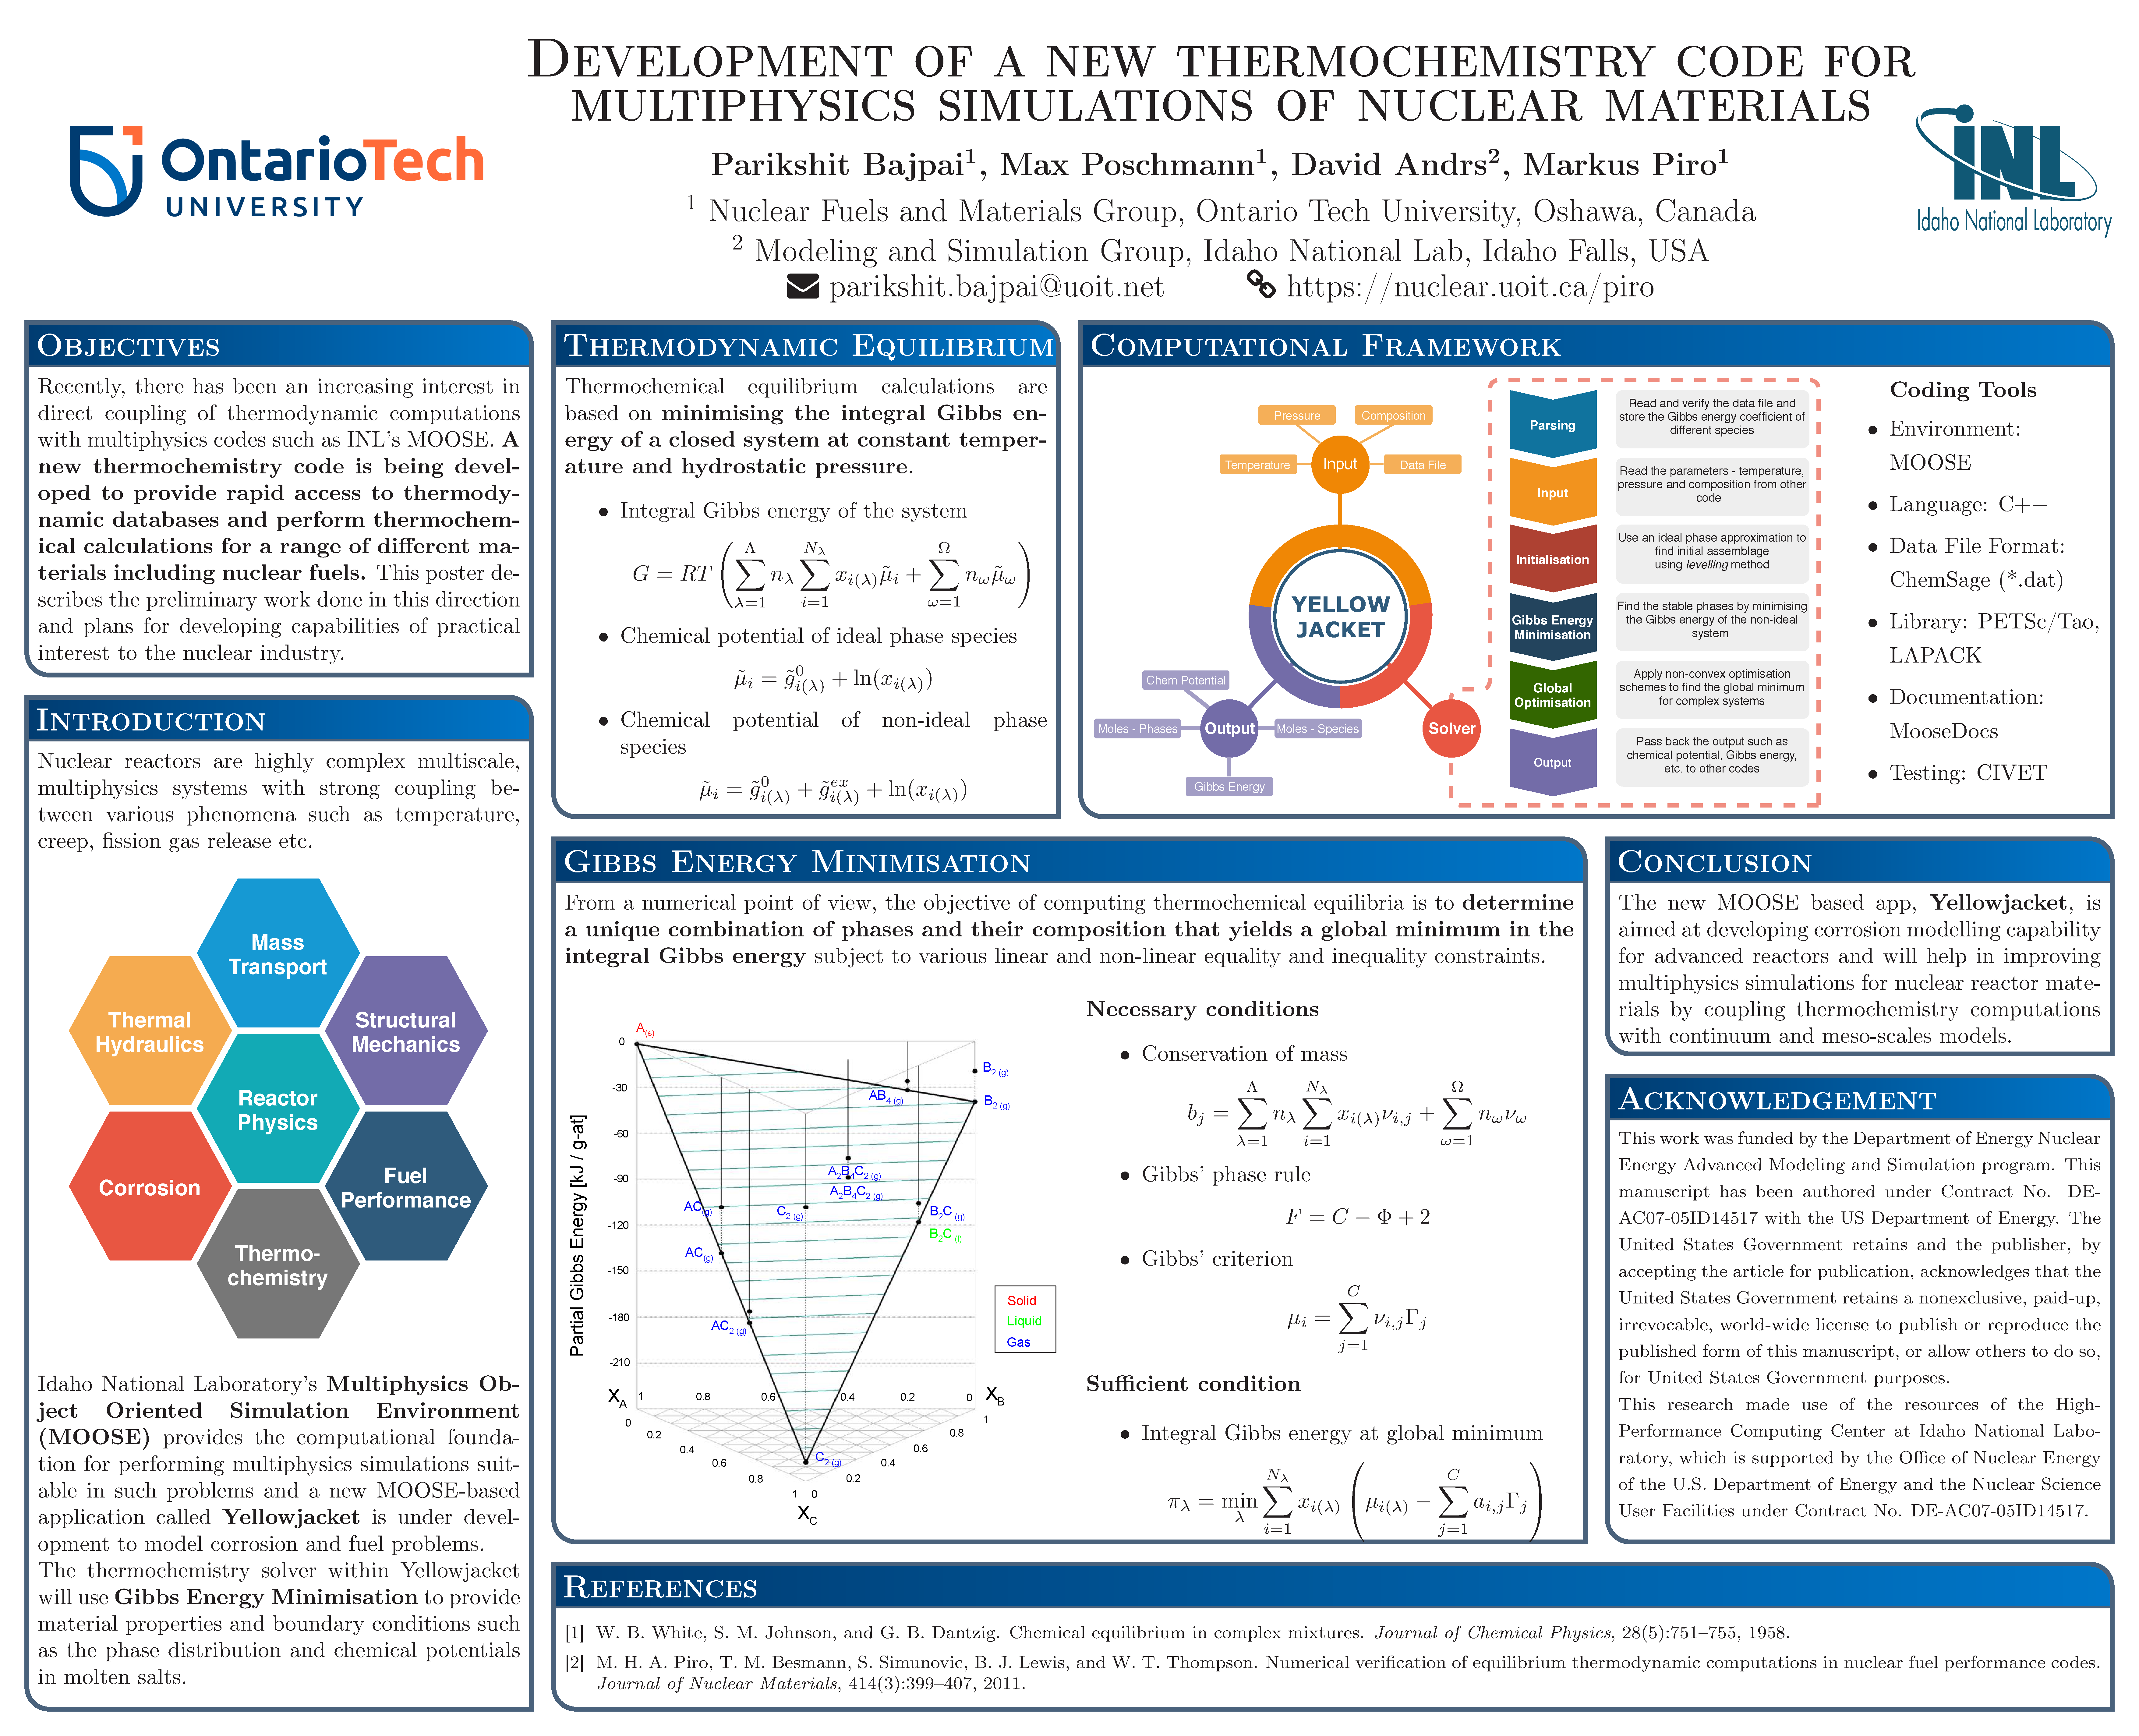
\includepdf[pages=-]{publications/CNS_Poster.pdf}
%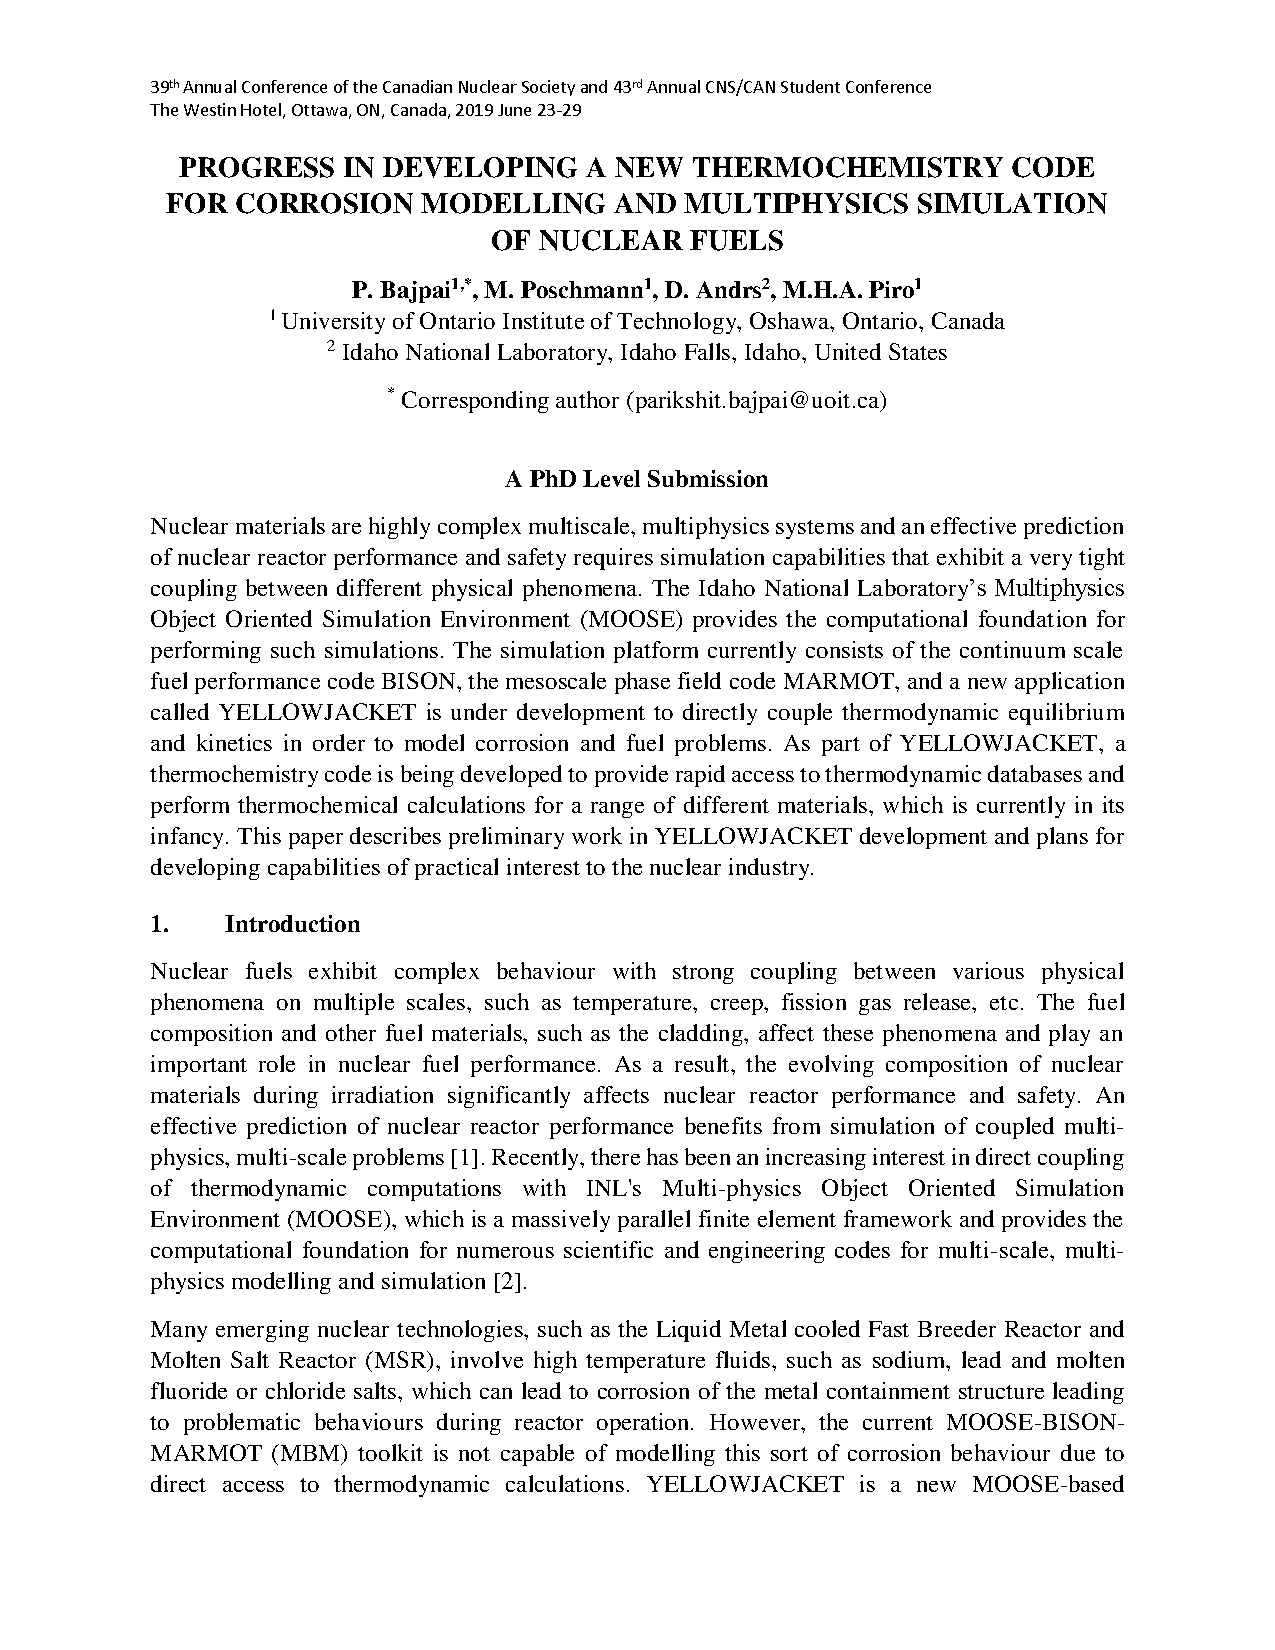
\includepdf[pages=-]{publications/Bajpai_2019.pdf}
%
%\setboolean{@twoside}{false}
}